\documentclass{article}
\usepackage{fullpage}
\usepackage{amsmath}
\usepackage{amssymb}
\usepackage{graphicx}
\usepackage{url, hyperref}

\renewcommand{\Pr}[1]{\mathbb{P}\left[#1\right]}
\newcommand{\Ex}[1]{\mathbb{E}\left[#1\right]}
\newcommand{\Var}[1]{\text{Var}\left[#1\right]}

\renewcommand{\bf}[1]{\mathbf{#1}}
\newcommand{\bs}[1]{\boldsymbol{#1}}
\newcommand{\mat}[1]{\ensuremath{\begin{pmatrix} #1 \end{pmatrix}}}


\begin{document}

Minqi Xu

20845758

m259xu

\subsection*{Question 1}

\begin{verbatim}
    close all;
    nSamples=2000;
    seed=758;
    rand('seed',seed);
    Ninside=0;
    rateInside=zeros(nSamples,1);

    for n=1:nSamples
     d=rand(1,1);
        x=4*d-2;
        d=rand(1,1);
        y=2*d-1;
        if((x^2+y^2)<=4)
            Ninside=Ninside+1;
        end
        rateInside(n)=Ninside/n
    end

    plot(rateInside,'r-','linewidth',2);
    title(sprintf('Rate of points inside ellipse (seed=%d)',seed));
    xlabel('Number of Points ploted');
    ylabel('Rate of Points inside ellipse');
    grid on

    pause

    print -dpsc2 dart.eps
    close
\end{verbatim}
\begin{figure}
    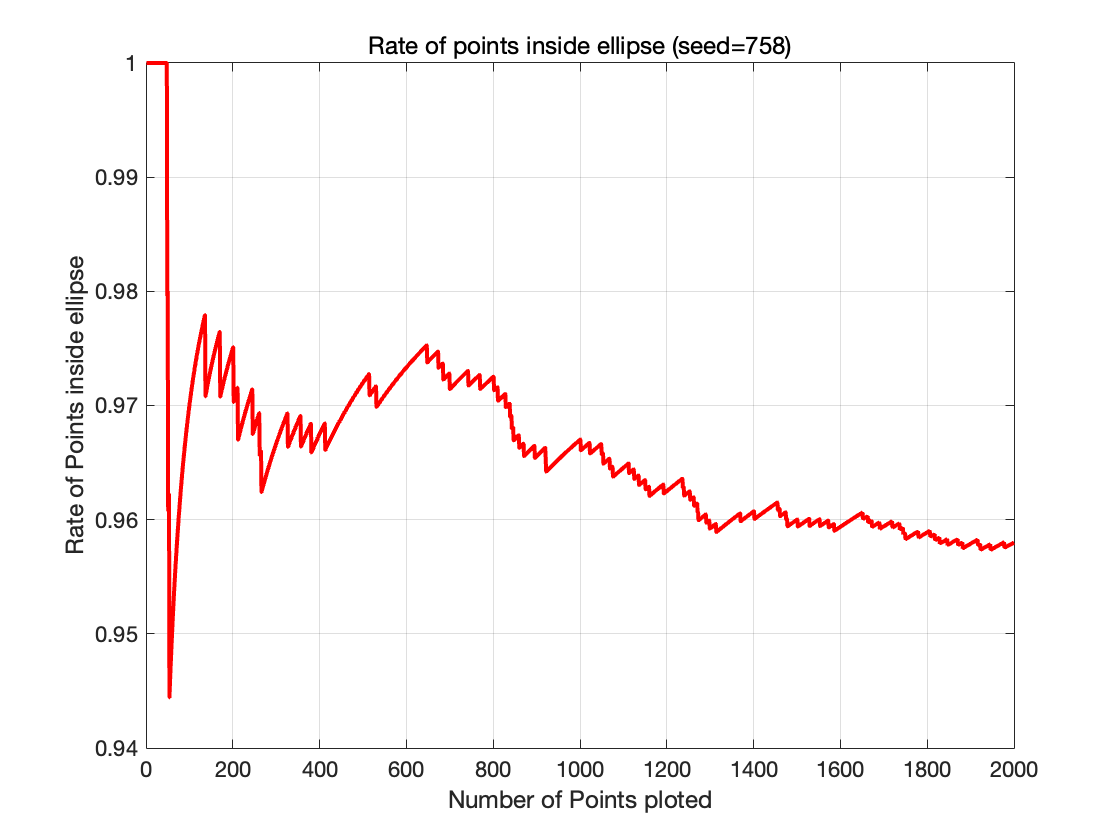
\includegraphics[width=\linewidth]{q1.png}
\end{figure}


\newpage
\subsection*{Question 2}
\begin{verbatim}
    close all;
    nSample=10000;
    seed=758;
    rand('seed',seed);
    Nsatisfied=0;
    proportion=0;

    for m=1:nSample
        d=rand(1,1);
        if((40*(d^2)+7)>(43*d))
            Nsatisfied=Nsatisfied+1;
        end
        if(m==1000)
            proportion=Nsatisfied/m;
            printf('Number of points = %d, proportion satisfied = %f',m,proportion)
        end
    end
    proportion=Nsatisfied/10000;
    sprintf('Number of points = 10000, proportion satisfied = %f',proportion)
\end{verbatim}
\begin{itemize}
    \item Number of points = 1000, proportion satisfied = 0.327000
    \item Number of points = 10000, proportion satisfied = 0.332400
\end{itemize}



\newpage
\subsection*{Question 3}
\begin{verbatim}
    close all;
    nSamples=10000;
    seed=758;
    rand('seed',seed);
    Ninside=0;
    Volumn=zeros(nSamples,1);

    for m=1:nSamples
       x=rand(1,1);
       y=rand(1,1);
       z=rand(1,1);
       if(((x^2+sin(y))<=z) & ((x-z+exp(y))<=1))
           Ninside=Ninside+1;
       end
       Volumn(m)=Ninside/m;
    end

    plot(Volumn,'r-','linewidth',2);
    title(sprintf('Volumn Approximations (seed=%d)',seed));
    xlabel('Number of Smaples');
    ylabel('Estimated Volumn');
    axis([1000,10000 0.1 0.2]);
    grid on

    pause
    print -dpsc2 volumn.eps
    close
\end{verbatim}
\begin{figure}
    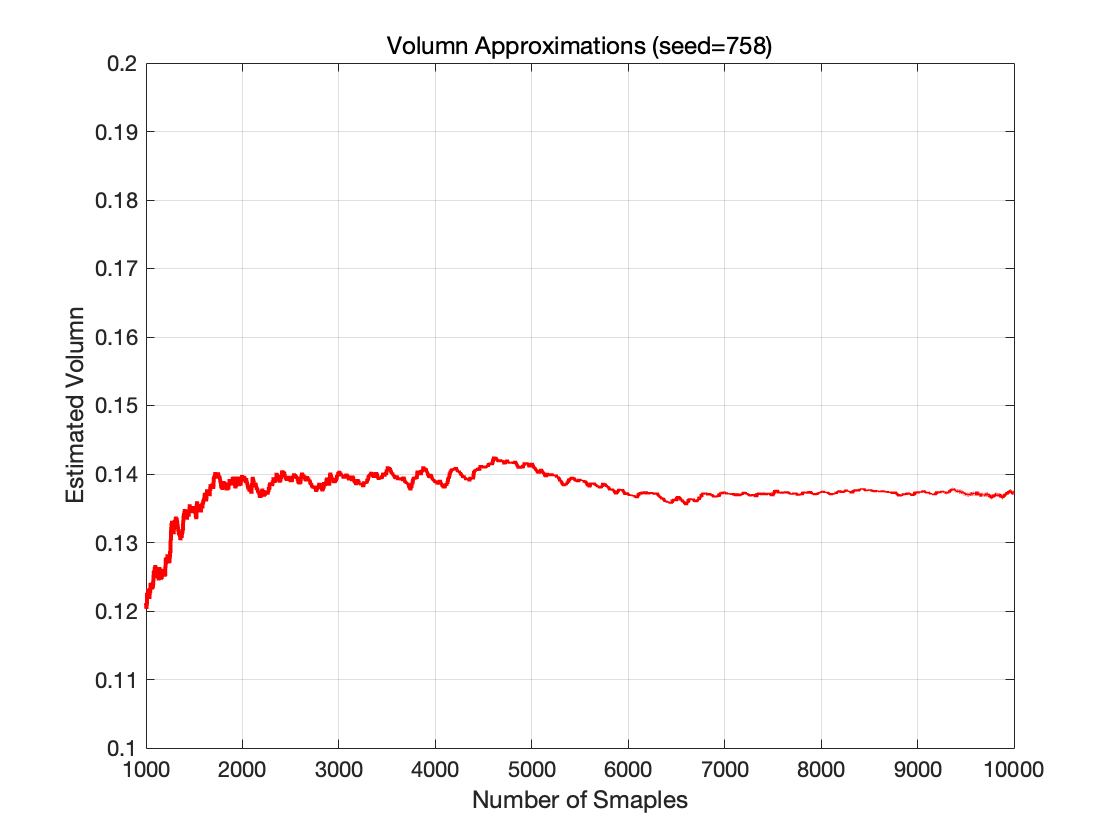
\includegraphics[width=\linewidth]{q3.png}
\end{figure}

\newpage
\subsection*{Question 4}
\begin{verbatim}
    close all;
    nSamples=100000;
    seed=758;
    rand('seed',seed);
    count=0;  % count stores the number of satisfied samples
    Pvalue=zeros(nSamples,1);  % Pvalue stores the probabilities wrt number of samples
    
    % Set the coordinate on the board, and assume that the two parallel lines
    %   are y=0 and y=1. Since the board are infinitely on x and y direction,
    %   therefore, when make a random point, x-value for the point is not 
    %   important, we only need to randomize the y-value of the point and the
    %   direction of the stick.
    for m=1:nSamples
        % we first random select the y-value of the center of the stick
        y=rand(1,1);
        % then we get the direction of the stick
        r=rand(1,1);
        % Due to the symmetry, we only need to random the direction in [0,pi)
        d=pi*r;
        % since the stick is unit long, only y(center)=0.5 and d=pi/2 can
        % intersects both parallel lines. We can separate the problem into 3
        % cases.
    
        % first case is y==0.5
        % this case, stick has no way to intersects one of the lines, thus
        % nothing changes.
    
        if(y>0.5)
            % in this case, stick can only intersects with the upper line, or
            % does not intersect with any lines.
            % len is the distance from center to the nearest line
            len = 1-y;
            % angle is the angle between the stick and the norm of the line
            angle = abs(pi/2 - d);
            if((0.5*cos(angle))>=len)
                % in this case stick intersects with the upper line
                count=count+1;
            end
        elseif(y<0.5)
            % similar to the previous case, but this time is lower line.
            % len is the distance from center to the nearest line
            len = y;
            % angle is the angle between the stick and the norm of the line
            angle = (pi/2 - d);
            if((0.5*cos(angle))>=len)
                % in this case stick intersects with the lower line
                count=count+1;
            end
        end
        % Pvalue stores the percentage, so 100 is multiplied
        Pvalue(m)=(count/m)*100;
    end
    
    plot(Pvalue,'r-','linewidth',2);
    title(sprintf('Probability stick intersects one of the lines (seed=%d)',seed));
    xlabel('Number of Samples');
    ylabel('Probability (%)');
    axis([1000,100000,60,70]);
    grid on
    
    pause
    print -dpsc2 prob.eps
    close
    
\end{verbatim}
\newpage
\begin{figure}
    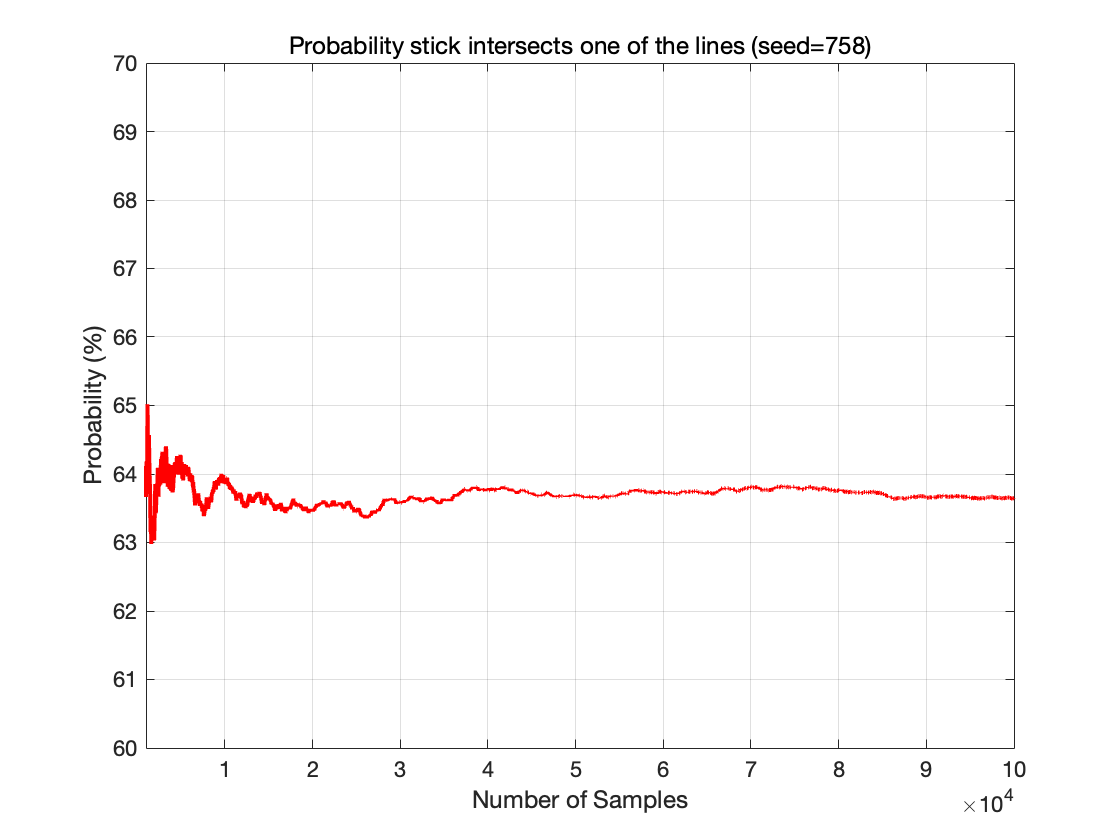
\includegraphics[width=\linewidth]{q4.png}
\end{figure}

\end{document}
